%\section*{Todesanzeigen}
\sectionmark{Todesanzeigen}

% Set thickness and padding of the frame
\setlength{\fboxsep}{3pt}  % No padding between the image and the frame
\setlength{\fboxrule}{1mm} % Thickness of the frame

%\begin{figure}[h!]
%	\begin{center}
%		\fbox{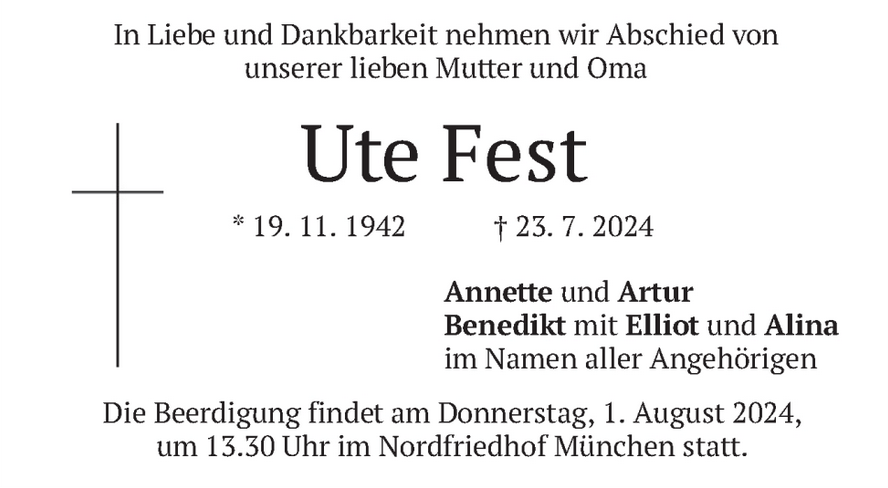
\includegraphics[width=.7\linewidth]{./Todesanzeigen/23.07.2024 Ute Fest.png}}
%		\vspace*{0.5cm}
%		\fbox{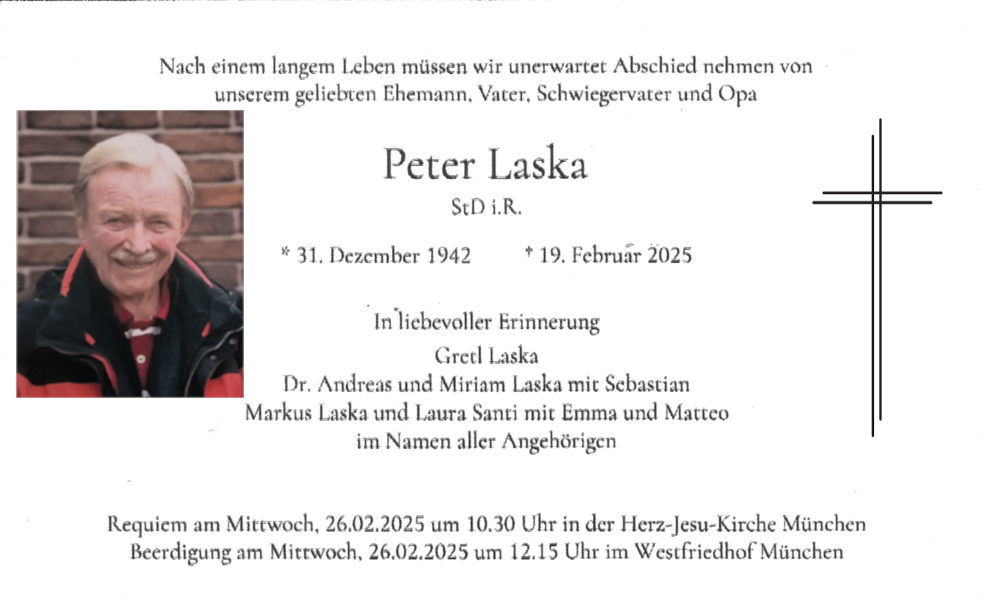
\includegraphics[width=.7\linewidth]{./Todesanzeigen/19.02.2025 PeterLaska.png}}
%	\end{center}
%\end{figure}
\begin{figure}[h!]
    \centering
    \fbox{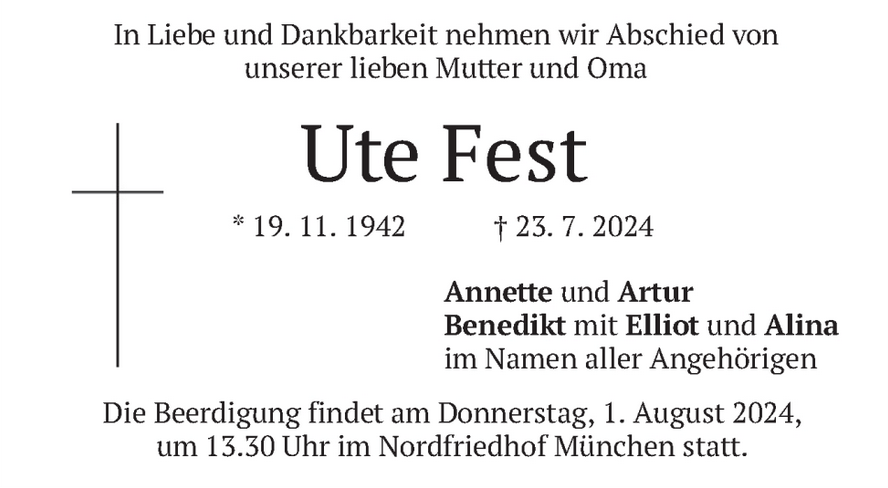
\includegraphics[width=.7\linewidth]{./Todesanzeigen/23.07.2024 Ute Fest.png}}
\end{figure}
    \vspace{0.4cm} % Should work better
\begin{figure}[h!]
    \centering
    \fbox{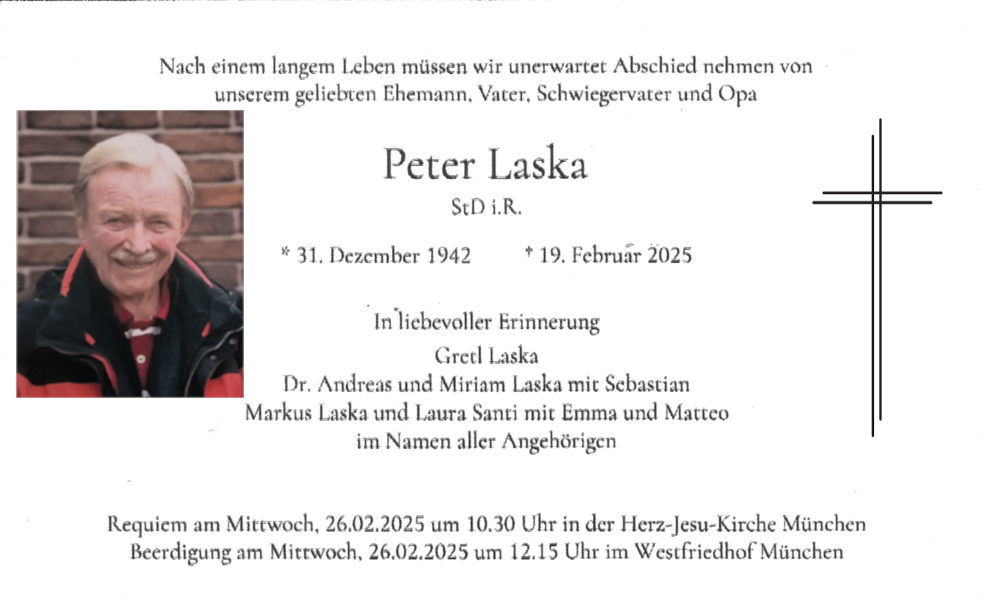
\includegraphics[width=.7\linewidth]{./Todesanzeigen/19.02.2025 PeterLaska.png}}
\end{figure}

\begin{multicols}{2}
			Am 26 Februar 2025 wurde unser Bundesbruder Peter Laska, StD i.R., im Familiengrab im Münchner Westfriedhof beigesetzt.
			Hier ruht auch sein Vater, unser hochverdienter Bundesbruder Josef Laska.
			Drei Chargierte der Aktivitas und einige Bundesbrüder erwiesen ihm die letzte Ehre und gaben ihm Band und Mütze als
			Dank und Zeichen der Verbundenheit mit ins Grab.
			Bundesbruder Peter Laska, geb. 1942 in Böhmen, wurde am 13.11.1964 von Vandalia rezipiert.
			Im WS 1965 war er Consenior der Aktivitas, 1966 Senior.
			Im Mai 1975 philistriert, übernahm er dennoch das anspruchsvolle Amt des Jubelseniors - 70 Jahre Vandalia! -
			 im Sommersemester 1975, um danach das Amt des Philisterconseniors weiterzuführen.
			61 Jahre lang hat Bbr. Peter Laska Vandalia die Treue gehalten. Ihm gebührt Vandalias besonderer Dank.
			REQUIESCAT IN PACE!
			\begin{flushright}
			\hfill\emph{Bernhard Müller Va!}
			\end{flushright}
\end{multicols}
